\scanpage{16}
Supposons en particulier
\[
B=A\otimes_k\Lambda
\]
où $\Lambda$ est une $k$-algèbre infinitésimale.
Alors \deleted{\unsure{on a} $\Omega^1_{\Lambda}$}
\[
\begin{aligned}
\unsure{\mathfrak g|\mathfrak T|\mathscr T|\mathcal T}_{B/\Lambda}\deleted{(B/\unsure{\Lambda|A})}
&=\mathrm{Hom}_B(\Omega^1_{B/\Lambda},B)\simeq\mathrm{Hom}_B(\Omega^1_{A/k}\otimes_k\Lambda,A\otimes_k\Lambda)\\
&\simeq\mathrm{Hom}_A(\Omega^1_{A/k},A\otimes_k\Lambda)\simeq k\text{-dérivations}\\
&\hspace{14em}\text{de }A\text{ dans }A\otimes_k\Lambda
\end{aligned}
\]
et les $\Lambda$-dérivations de $B$ dans $B$ qui
induisent $0$ sur $B\otimes_\Lambda k\simeq\Lambda$ s'identifient
aux $k$-dérivations $A\unsure{\text{—}|\longrightarrow} A\otimes_k I(\Lambda)$.

Donc

\uline{Proposition} Supposons $k$ \deleted{\unsure{de car.}} $\inserted{\supset}\mathbb Q$, $A$ une
\reversemarginpar\margin{\hfill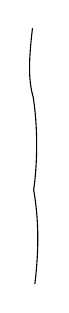
\begin{tikzpicture}[x=3mm,y=5mm]
\draw (0,0) .. controls (-.18,-.9) and (-.16,-1.35) .. (.03,-1.75) .. controls (.30,-2.80) and (.13,-3.80) .. (.05,-4.10) .. controls (.20,-4.65) and (.33,-5.35) .. (.10,-6.5);
\end{tikzpicture}}\normalmarginpar
$k$-alg. comm., $\Lambda$ une $k$-alg. \unsure{diff.|dpf.}
Alors le \inserted{groupe des} $\Lambda$-aut.m. infinitésimaux de
$A\otimes_k\Lambda$ \deleted{\unsure{sont en co}} est isomorphe
à l'ens des $k$-dérivations de
$A$ dans $A\otimes_k I(\Lambda)$, avec la structure
de groupe donnée par Hausdorff-Campbell.
% archive sheet number: 15

